\chapter{PlantaBot - Um Sistema Especialista para Supervisão e Manutenção de Planta Industrial}

\begin{flushright}
Sid Gubert
\end{flushright}

PlantaBot é um Assistente Virtual Especialista em Supervisão e Manutenção Preditiva de Planta Industrial, integrado ao ecossistema supervisório \textit{PlantaView}. O seu objetivo é auxiliar operadores de sala de controle, técnicos e engenheiros de manutenção no diagnóstico em tempo real de anomalias operacionais, na interpretação de grandezas físicas (temperatura, pressão, vazão e vibração mecânica) e na priorização de ordens de serviço.

Nos sistemas supervisórios industriais do tipo SCADA (\textit{Supervisory Control and Data Acquisition}), o volume contínuo de telemetria e a ocorrência simultânea de eventos de alarme exigem respostas rápidas e precisas para evitar paradas não programadas ou danos severos a ativos críticos \cite{mobley2002introduction}. A integração de Sistemas Especialistas baseados em Grandes Modelos de Linguagem (LLMs) com bases de conhecimento normativas, como os critérios de severidade de vibração da norma ISO 10816 \cite{iso10816} e protocolos de bloqueio de segurança LOTO (\textit{Lockout/Tagout}), permite transformar dados brutos de sensores em recomendações prescritivas acionáveis \cite{yang2025comprehensive,garridomerchan2026gofai}.

O desenvolvimento do PlantaBot uniu a inferência local via modelos de linguagem executados no servidor \textit{Ollama} com a consulta determinística a ferramentas industriais via protocolo MCP (\textit{Model Context Protocol}). A solução utiliza \textit{prompts} estruturados para configurar uma persona especialista em engenharia de manutenção industrial, disponibilizando uma interface conversacional (\textit{chat}) capaz de correlacionar histórico de sensores, alarmes ativos e ordens de manutenção.

As seções seguintes descrevem a arquitetura do sistema, o conjunto de ferramentas MCP desenvolvidas para inspeção da planta, o fluxo de implementação e validação automatizada e as instruções para reprodução e reuso da solução.

\section{Arquitetura do PlantaBot}

A Figura \ref{fig:arquitetura-plantabot} apresenta a arquitetura de interfaces e componentes do PlantaBot. O operador interage com o núcleo do Sistema Especialista por meio de uma interface de \textit{chat}. Ao receber uma consulta, o sistema verifica inicialmente a aderência ao domínio industrial (\textit{guardrails} de escopo) e consulta a memória de trabalho. O núcleo de inferência é composto por um LLM local servido via \textit{Ollama} (\texttt{qwen2.5:1.5b} ou \texttt{qwen3:4b}), parametrizado por um \textit{prompt} de sistema que incorpora as regras operacionais e os procedimentos de manutenção da base de conhecimento (\path{conhecimento/planta.json}), abstendo-se de responder a questões alheias à operação da planta industrial. A memória de trabalho combina dois mecanismos complementares: (i) um cache semântico vetorial, capaz de recuperar instantaneamente respostas para perguntas semanticamente equivalentes a consultas já processadas (distância de cosseno $\le 0{,}20$), e (ii) o histórico conversacional mantido na sessão de inferência junto ao motor LLM.

\begin{figure}[htbp]
\centering
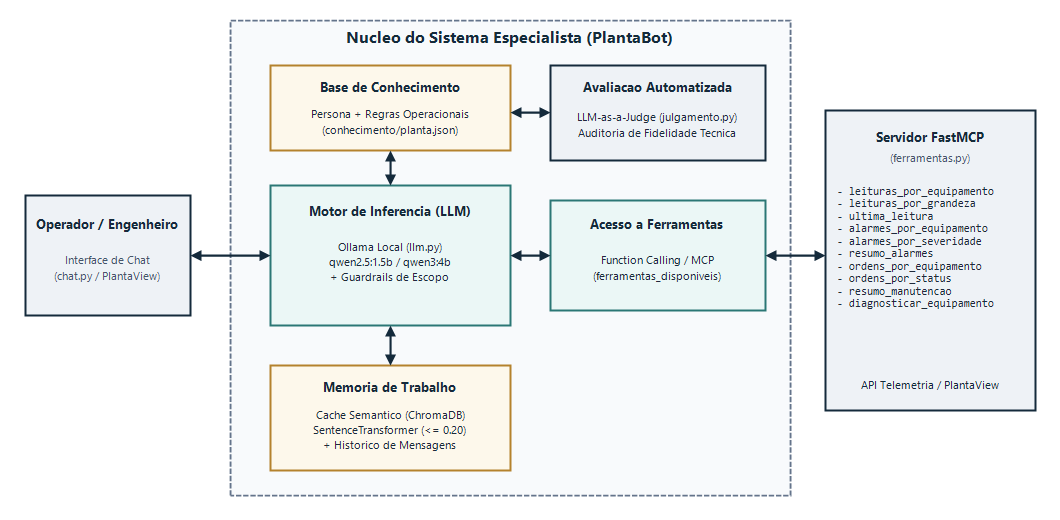
\includegraphics[width=1.0\textwidth]{capitulos/capitulo_2/arquitetura.png}
\caption{Arquitetura do PlantaBot}
\label{fig:arquitetura-plantabot}
\end{figure}

\section{Ferramentas MCP}

Por meio do protocolo MCP \cite{mcp2026architecture}, o PlantaBot conecta o motor de inferência diretamente aos dados operacionais dos ativos monitorados na planta industrial (Bomba Centrífuga Principal \texttt{EQ-001}, Compressor de Ar Industrial \texttt{EQ-002}, Caldeira de Vapor \texttt{EQ-003}, Torre de Resfriamento \texttt{EQ-004} e Motor Elétrico Trifásico \texttt{EQ-005}). Dessa forma, sempre que o operador questiona o estado atual de um equipamento, o modelo invoca automaticamente a ferramenta apropriada (\textit{function calling}) e fundamenta seu parecer técnico nos indicadores reais da planta.

O servidor MCP do PlantaBot disponibiliza dez ferramentas organizadas em quatro categorias operacionais: (i) monitoramento de sensores: \path{leituras_por_equipamento}, \path{leituras_por_grandeza} e \path{ultima_leitura}, que retornam séries históricas, estatísticas (mínimo, máximo, média e tendência por hora) e limites operacionais de cada sensor; (ii) gestão de alarmes: \path{alarmes_por_equipamento}, \path{alarmes_por_severidade} e \path{resumo_alarmes}, que filtram eventos ativos ou reconhecidos segundo a criticidade (\texttt{CRITICO}, \texttt{ALTO}, \texttt{MEDIO} e \texttt{BAIXO}); (iii) controle de manutenção: \path{ordens_por_equipamento}, \path{ordens_por_status} e \path{resumo_manutencao}, que consultam ordens de serviço preventivas e corretivas; e (iv) diagnóstico integrado: \path{diagnosticar_equipamento}, que consolida leituras em anomalia, tendência térmica/mecânica, alarmes ativos e ordens pendentes para emitir um laudo completo do ativo.

\section{Desenvolvimento e Avaliação}

O PlantaBot foi implementado em linguagem Python, integrando bibliotecas voltadas à recuperação semântica, inferência em LLMs e exposição de serviços MCP. A biblioteca \textit{sentence-transformers} (\texttt{paraphrase-multilingual-MiniLM-L12-v2}) converte tanto as regras da base de conhecimento quanto as dúvidas dos operadores em vetores densos (\textit{embeddings}), os quais são persistidos e consultados na base vetorial \textit{chromadb}. A comunicação com o motor de inferência local no \textit{Ollama} é realizada pelo módulo \path{llm.py}, que gerencia o envio de contexto, a remoção automática de blocos intermediários de raciocínio (\textit{thinking tags}) e o ciclo de invocação das ferramentas registradas via \texttt{FastMCP} (\path{ferramentas.py}).

A Figura \ref{fig:funcionamento-plantabot} ilustra o funcionamento do PlantaBot em execução. Observa-se tanto o acionamento automático da ferramenta MCP \path{diagnosticar_equipamento} para inspecionar a Bomba Centrífuga Principal (\texttt{EQ-001}) quanto a recuperação imediata pelo cache semântico em consultas normativas sobre faixas operacionais.

\begin{figure}[htbp]
\centering
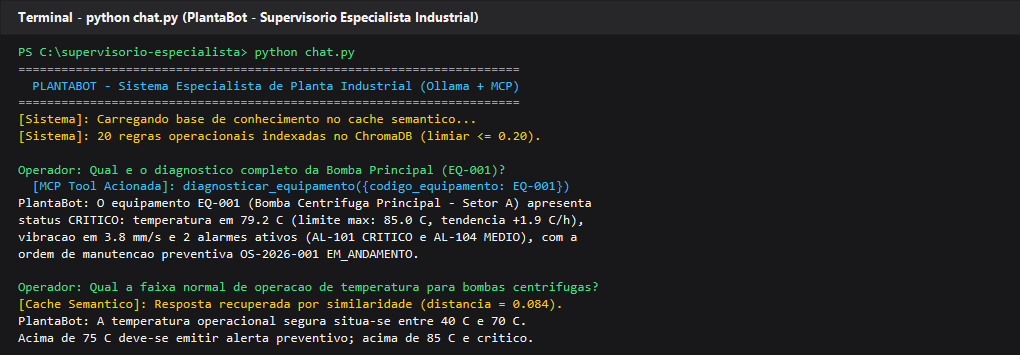
\includegraphics[width=1.0\textwidth]{capitulos/capitulo_2/funcionamento.png}
\caption{Funcionamento do PlantaBot}
\label{fig:funcionamento-plantabot}
\end{figure}

Para aferir de forma sistemática a qualidade e a fidelidade técnica das respostas geradas pelo especialista, aplicou-se a técnica \textit{LLM-as-a-Judge} \cite{azevedo2026julgamento} por meio do script \path{julgamento.py}. Nessa etapa, o modelo especialista (\texttt{qwen2.5:1.5b}) responde às questões de referência da planta industrial sem auxílio do cache pré-carregado, enquanto um modelo julgador independente de maior capacidade (\texttt{qwen3:4b}) avalia cada resposta gerada em comparação ao gabarito de engenharia de manutenção, classificando-a como adequada ou inadequada com justificativa técnica. O resultado da avaliação automatizada é apresentado na Figura \ref{fig:julgamento-plantabot}.

\begin{figure}[htbp]
\centering
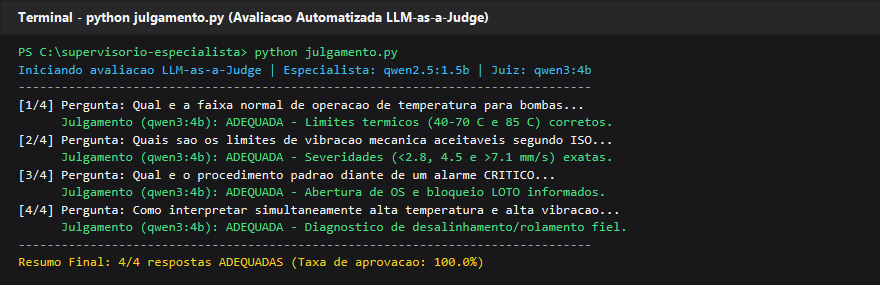
\includegraphics[width=1.0\textwidth]{capitulos/capitulo_2/julgamento.png}
\caption{Julgamento do PlantaBot}
\label{fig:julgamento-plantabot}
\end{figure}

\section{Reproducibilidade e Reuso}

O código-fonte completo do PlantaBot (Supervisório Especialista), incluindo a base de conhecimento industrial, o servidor de ferramentas MCP, os testes automatizados e o avaliador \textit{LLM-as-a-Judge}, pode ser consultado e (re)usado livremente através do link de acesso ao \href{https://zenodo.org/records/supervisorio-especialista?preview_file=supervisorio-especialista.zip}{repositório do projeto} (também disponível em \url{https://github.com/sidgubert/supervisorio-especialista}). Também se encontra disponibilizado um vídeo demonstrativo \href{https://zenodo.org/records/supervisorio-especialista/preview/plantabot.mp4}{neste link}.
